
\chapter{}
\newpage

\section[Fiche technique vernis Lascaux]{Fiche technique vernis Lascaux transparent 1-UV}\label{fiche_technique_Lascaux}

\begin{figure}[H]
    \centering
    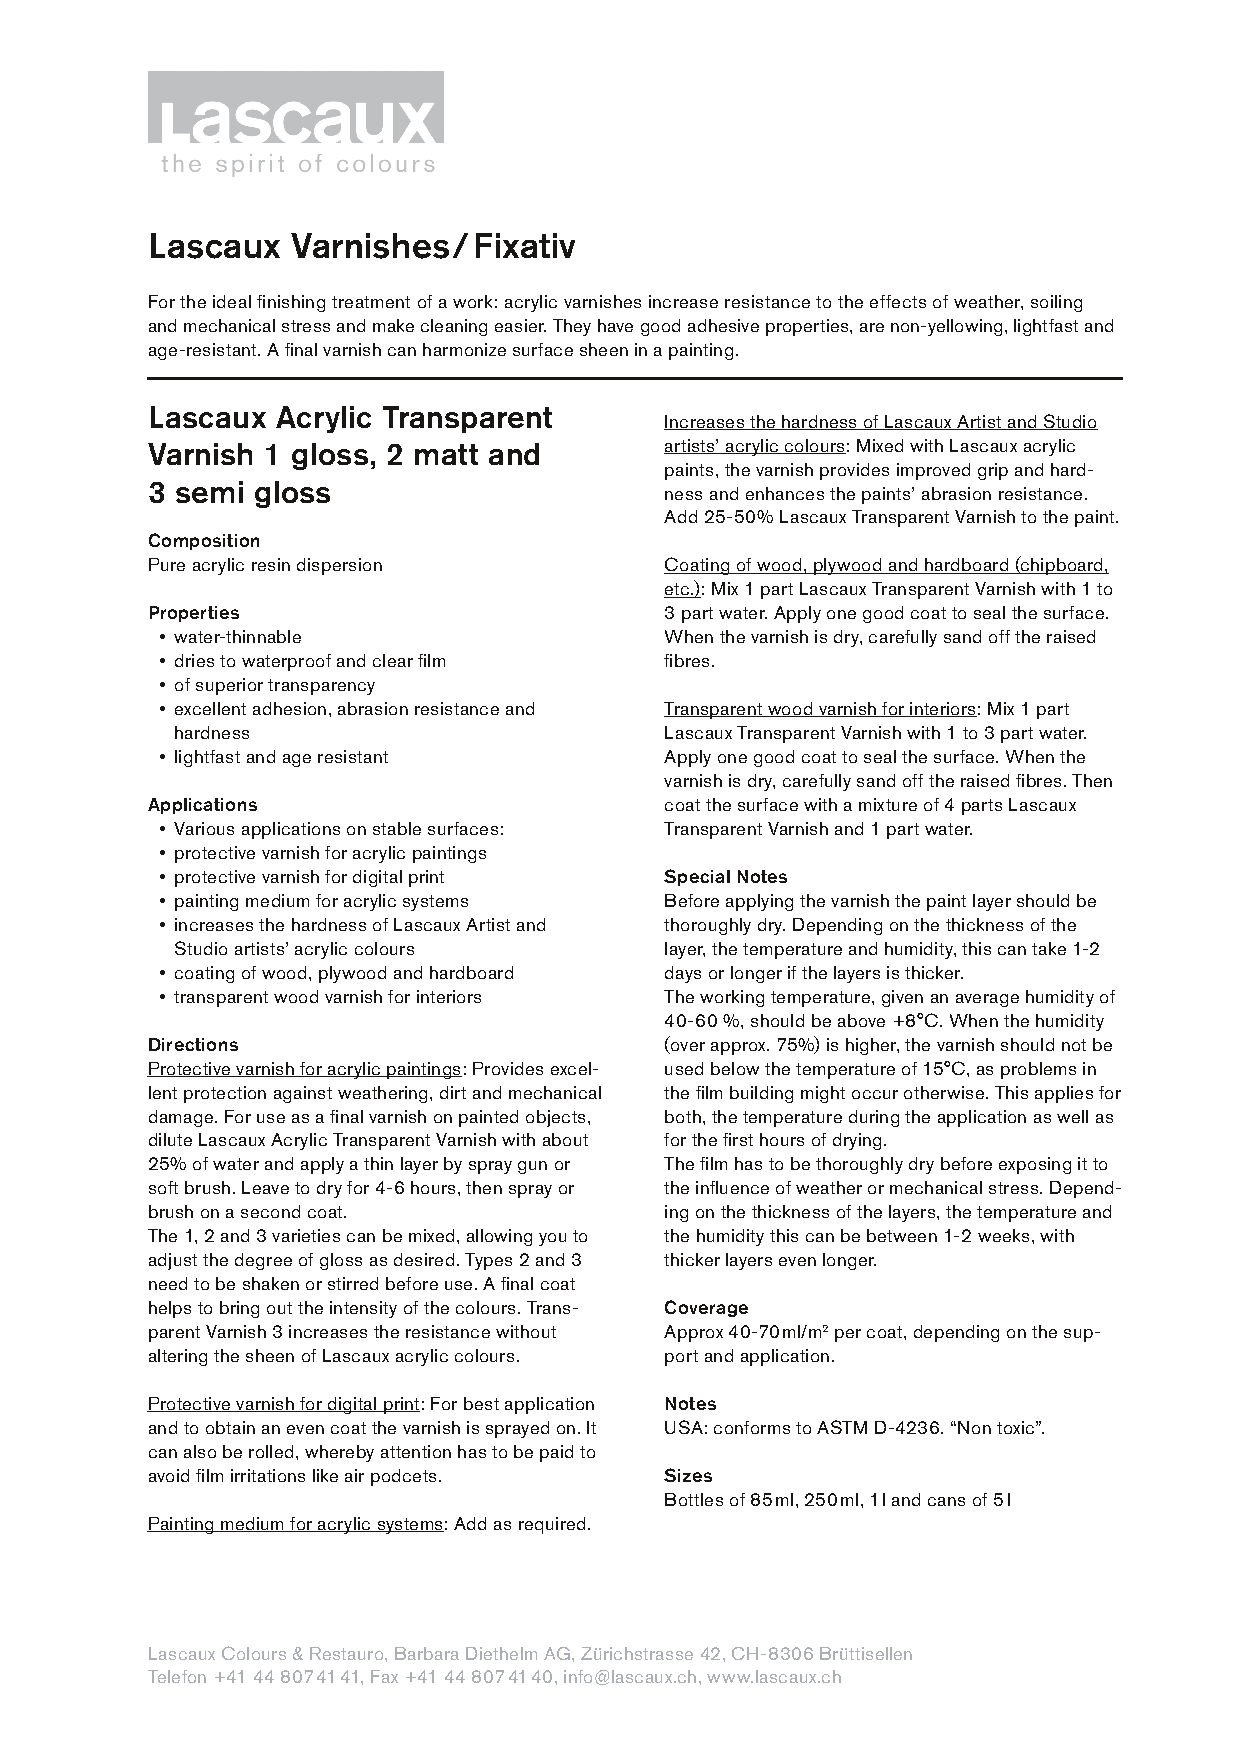
\includepdf[pages=1,scale=0.9,pagecommand={}]{assets/Annexes/Lascaux Varnishes_Fixative.pdf}
    %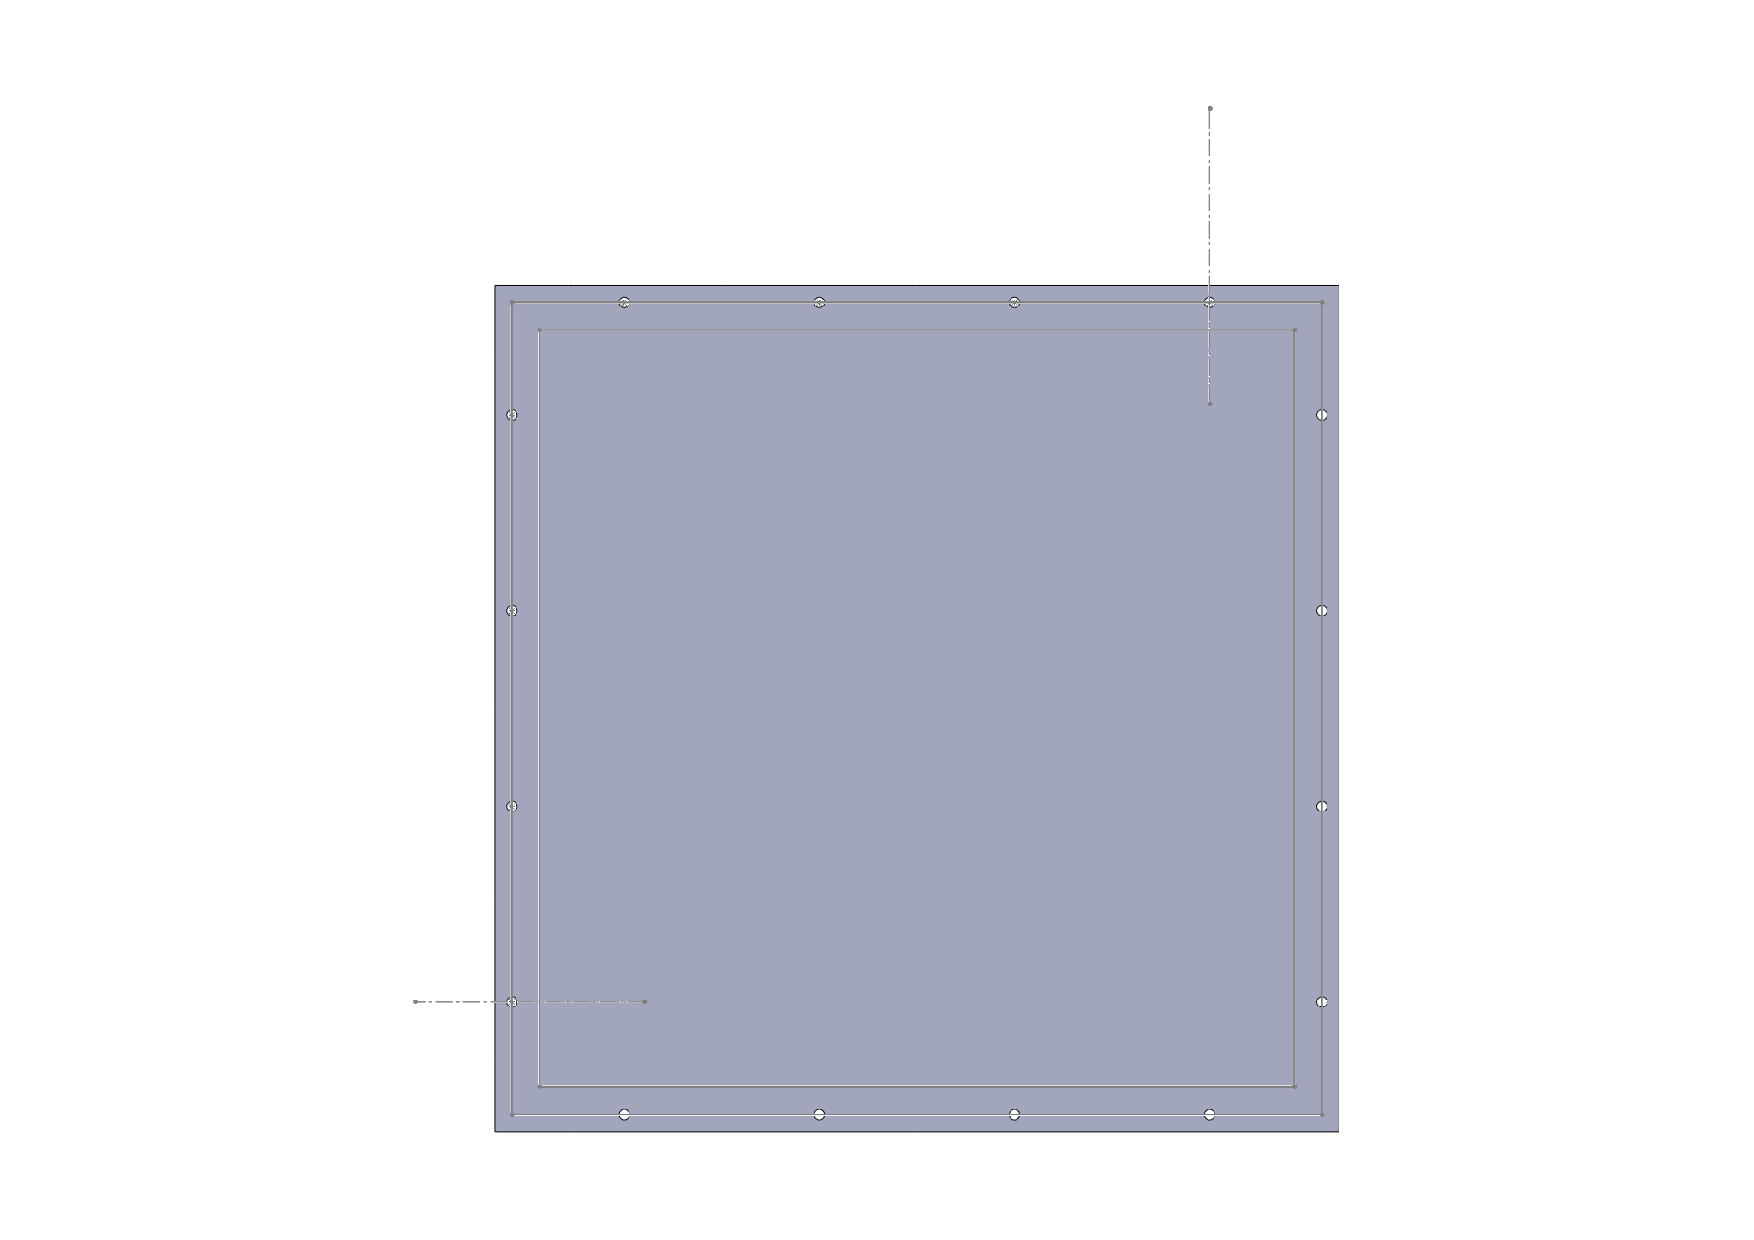
\includegraphics[width = \textwidth]{assets/Annexes/chablon trous.pdf}
\end{figure}
\includepdf[pages=2-,scale=0.9,pagecommand={}]{assets/Annexes/Lascaux Varnishes_Fixative.pdf}

\section[Fiche technique Lascaux spécifique UV]{Fiche technique Lascaux spécifique UV}\label{fiche_technique_Lascaux_UV}

\begin{figure}[H]
    \centering
    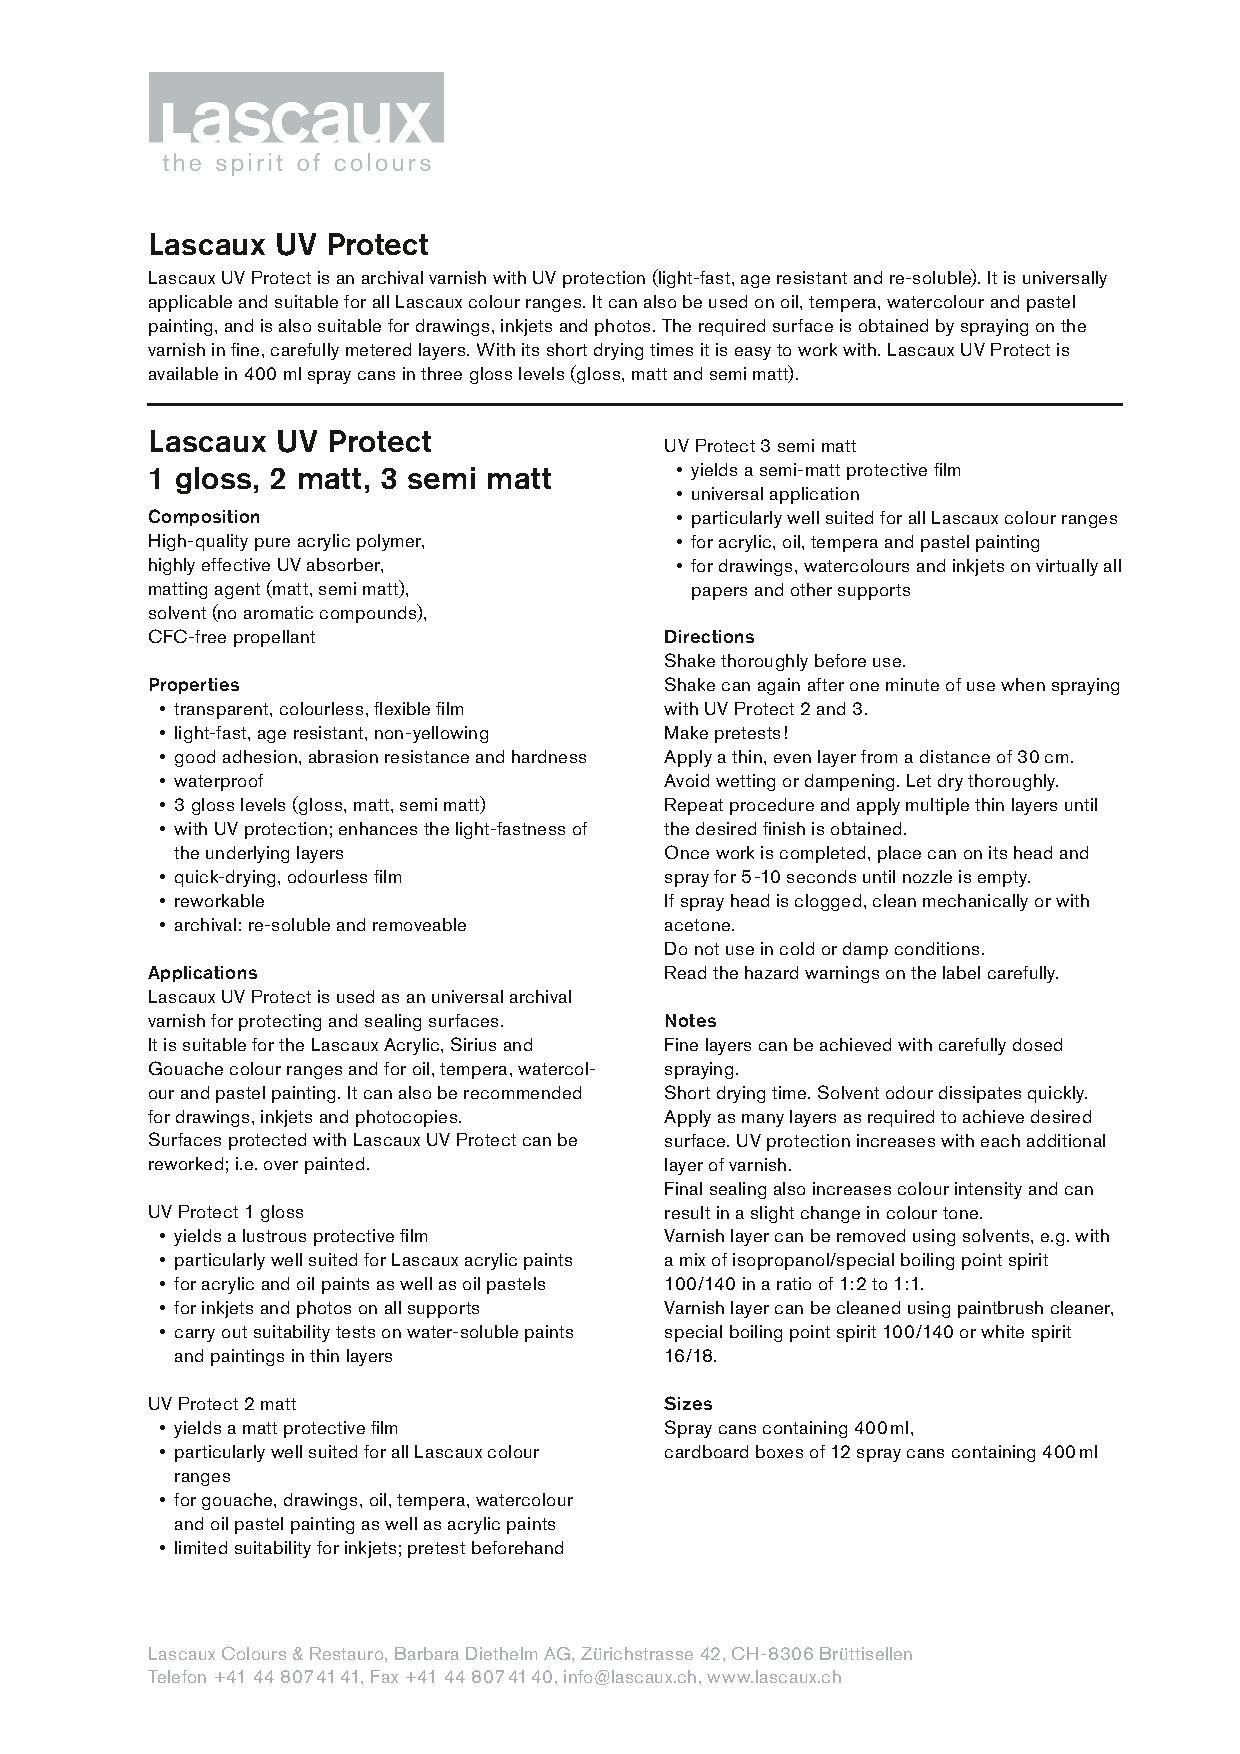
\includepdf[pages=1,scale=0.9,pagecommand={}]{assets/Annexes/Lascaux_UV_Protect_E.pdf}
    %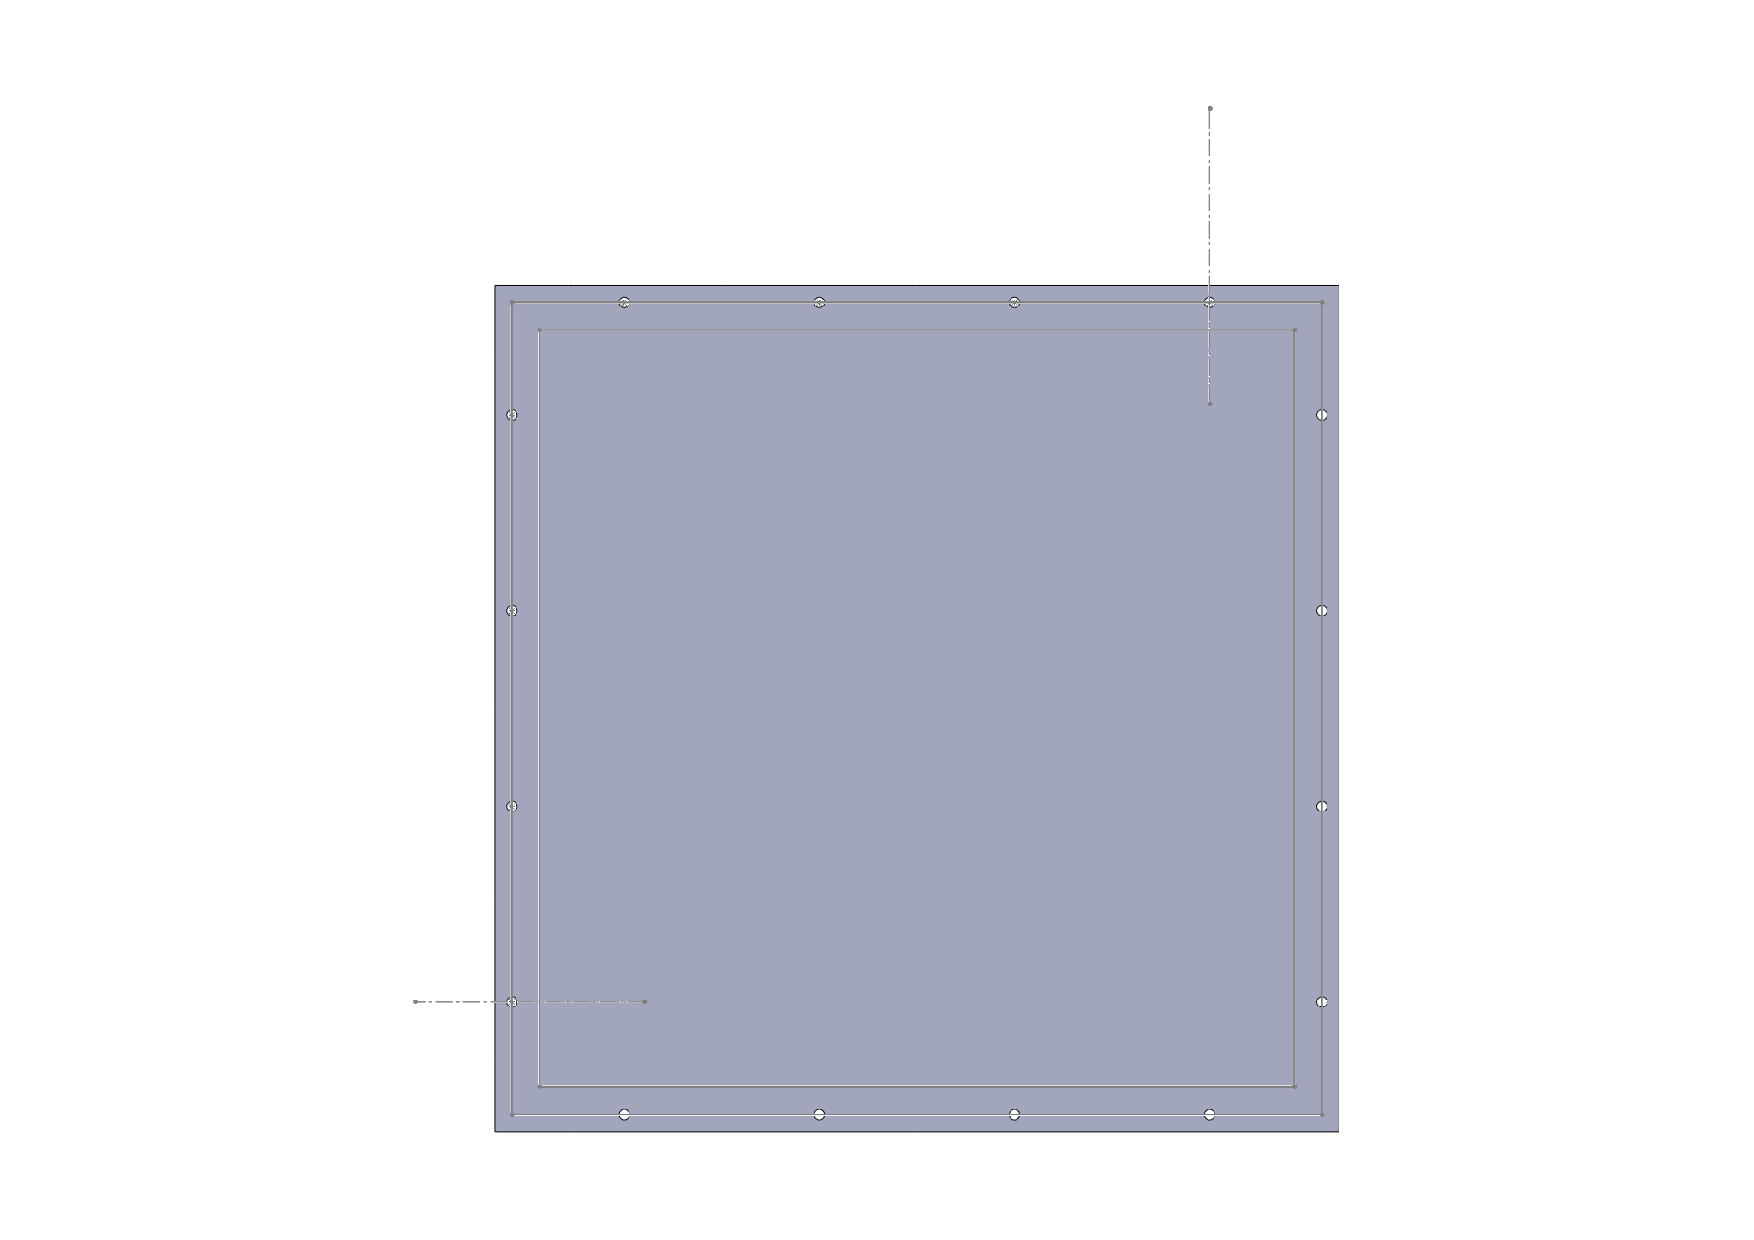
\includegraphics[width = \textwidth]{assets/Annexes/chablon trous.pdf}
\end{figure}
\includepdf[pages=2-,scale=0.9,pagecommand={}]{assets/Annexes/Lascaux_UV_Protect_E.pdf}


\section[Fiche technique Stardust Colors]{Fiche technique Top coats Stardust Colors}\label{fiche_technique_Stardust}

\begin{figure}[H]
    \centering
    
\includepdf[pages=6,scale=0.7,angle=90,pagecommand={}]{assets/Annexes/Catalog_STARDUST PRO_UK.pdf}
    %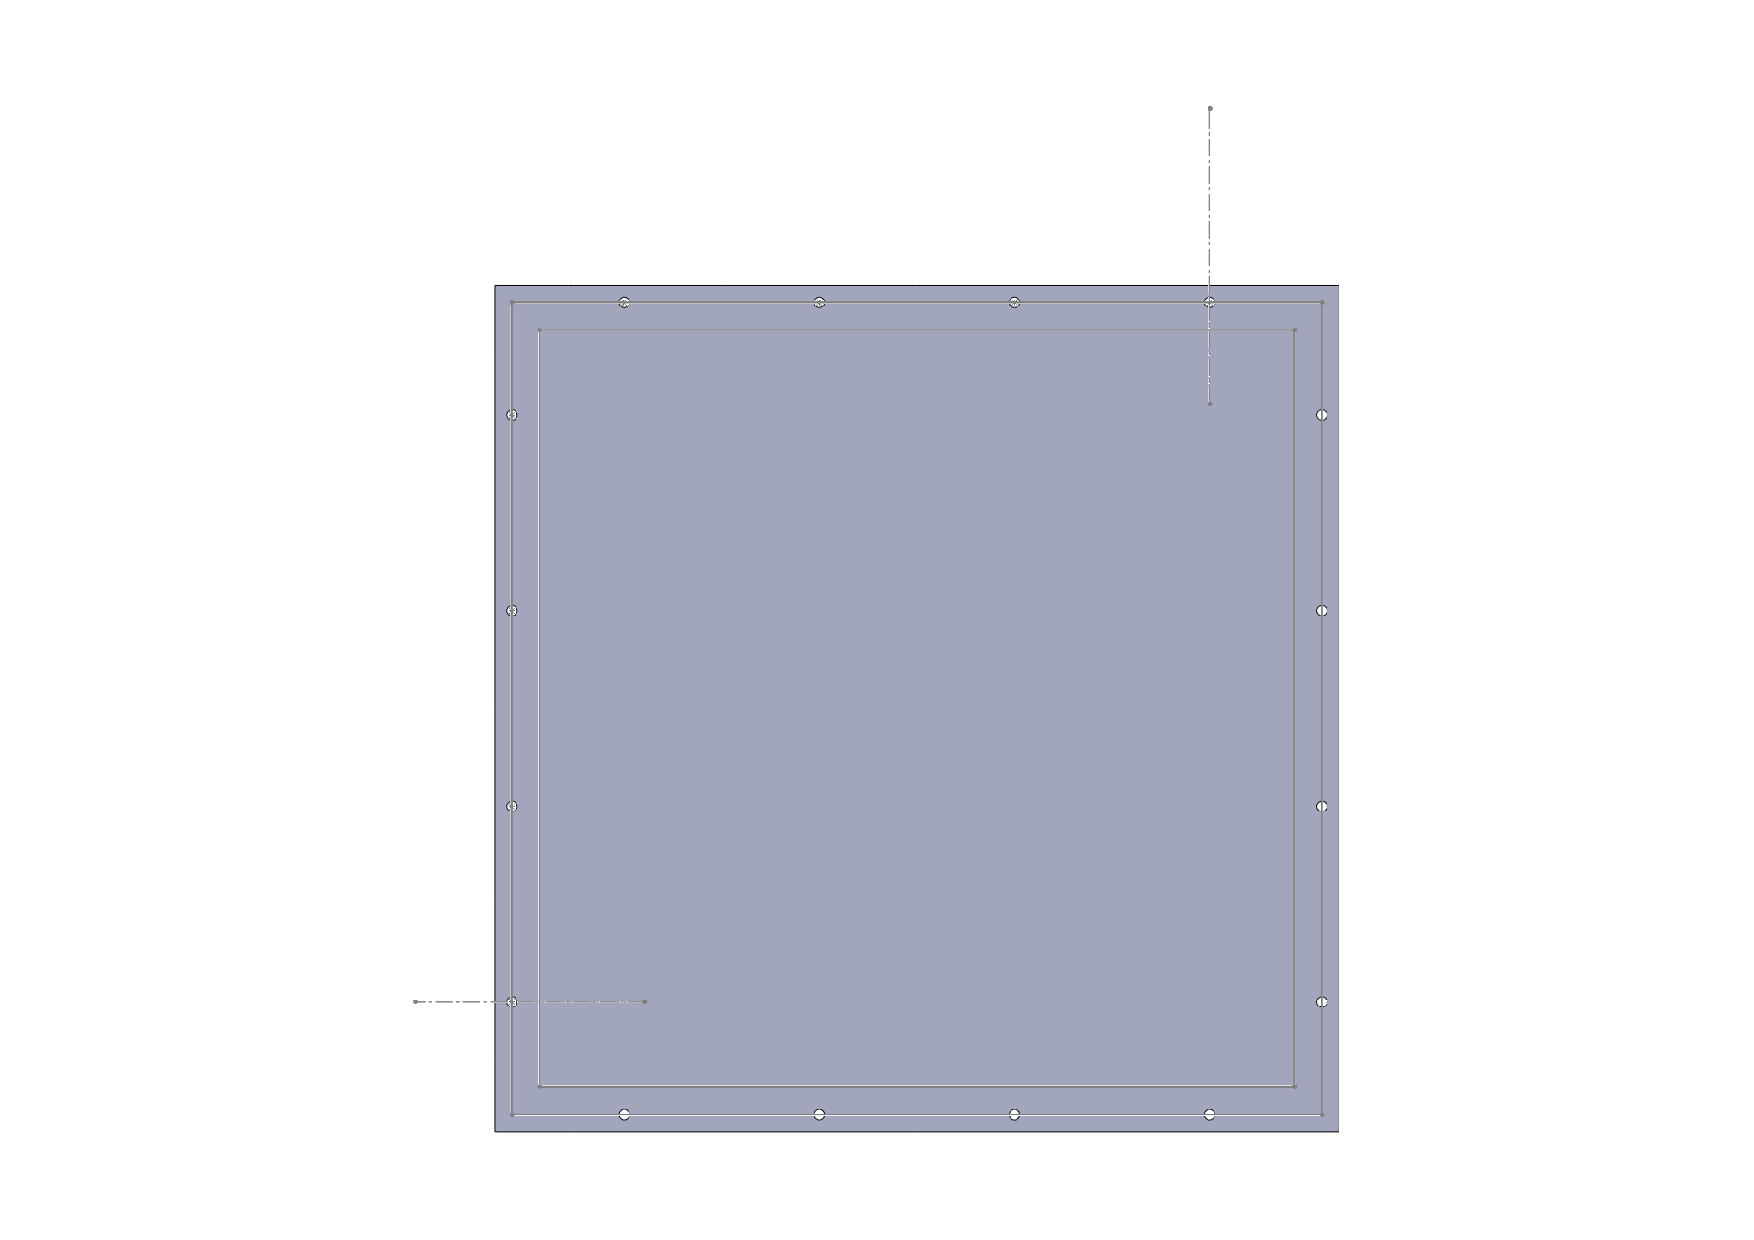
\includegraphics[width = \textwidth]{assets/Annexes/chablon trous.pdf}
\end{figure}


\newpage
\section[Fiche technique vernis Createx]{Fiche technique vernis Createx}\label{fiche_technique_Createx}

\begin{figure}[H]
    \centering
    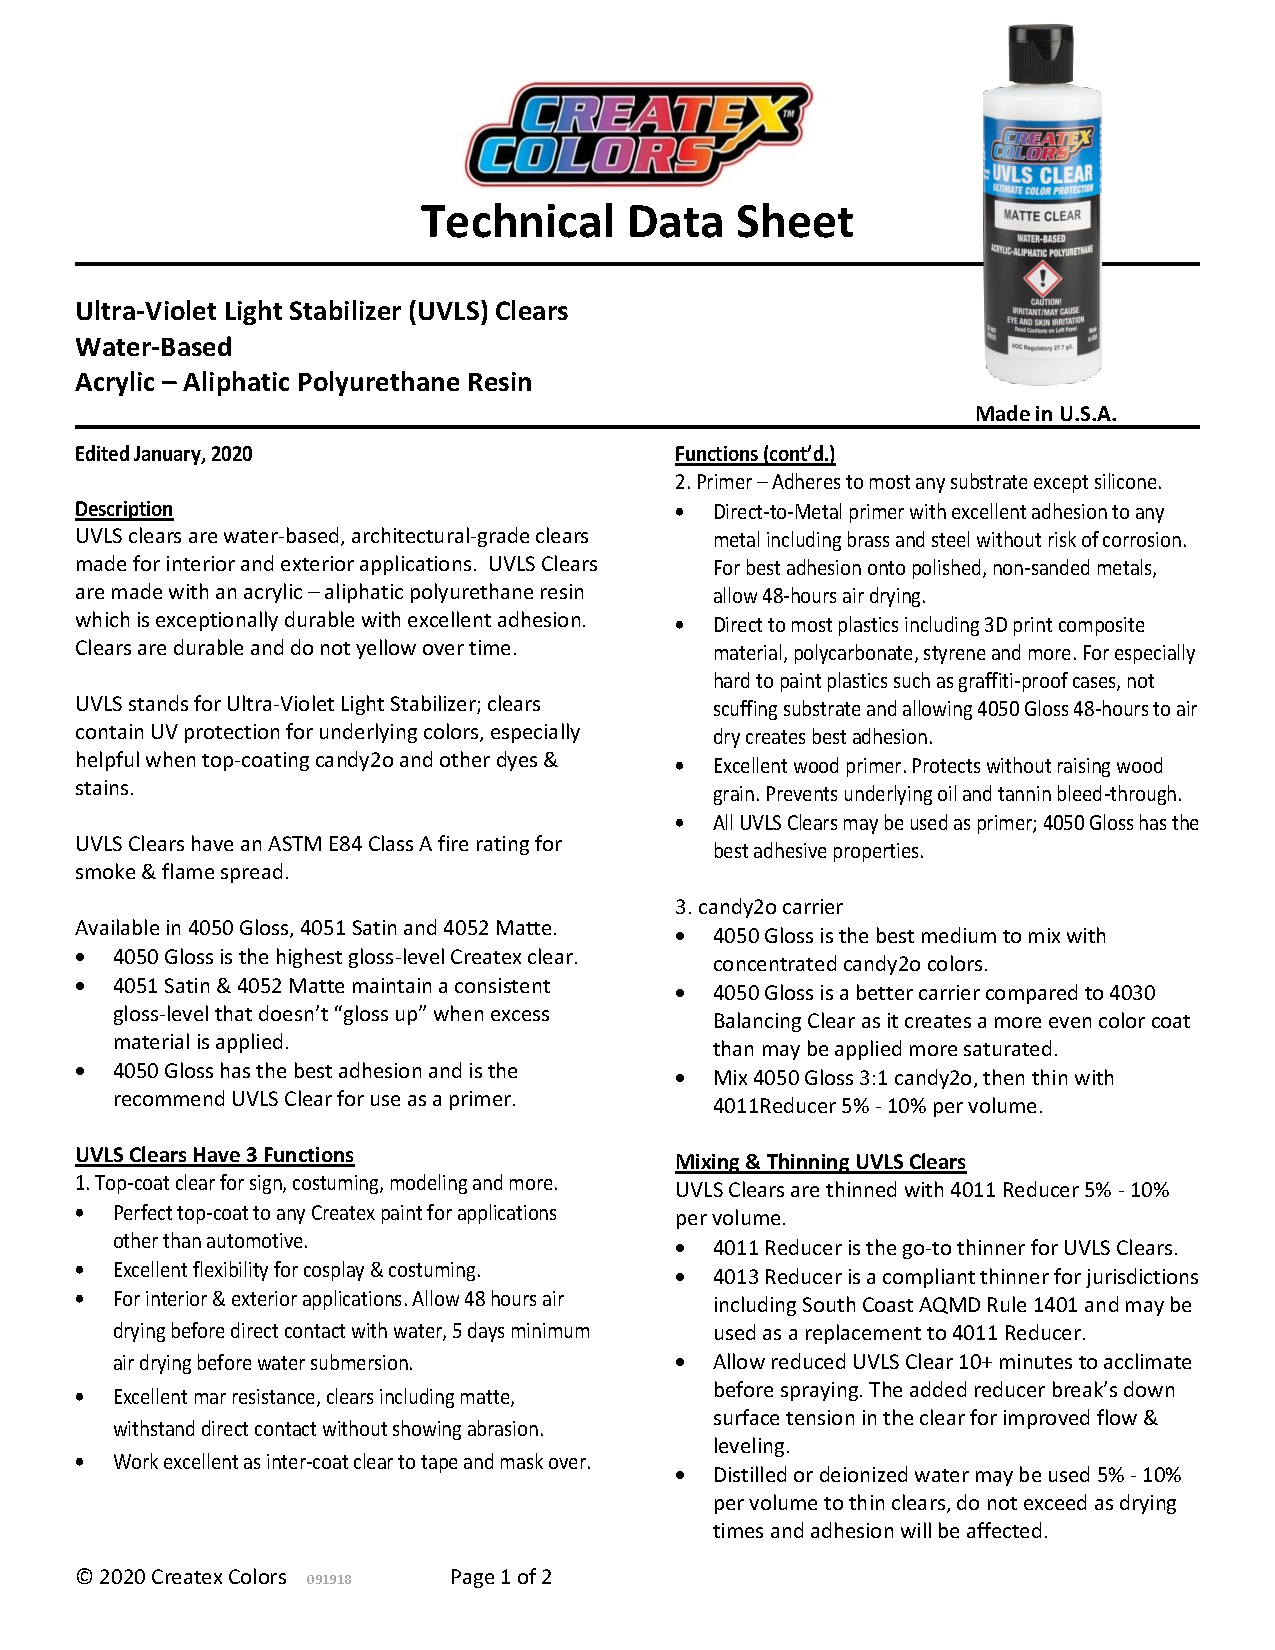
\includepdf[pages=1,scale=0.8,pagecommand={}]{assets/Annexes/UVLS-Clears-TDS.pdf}
    %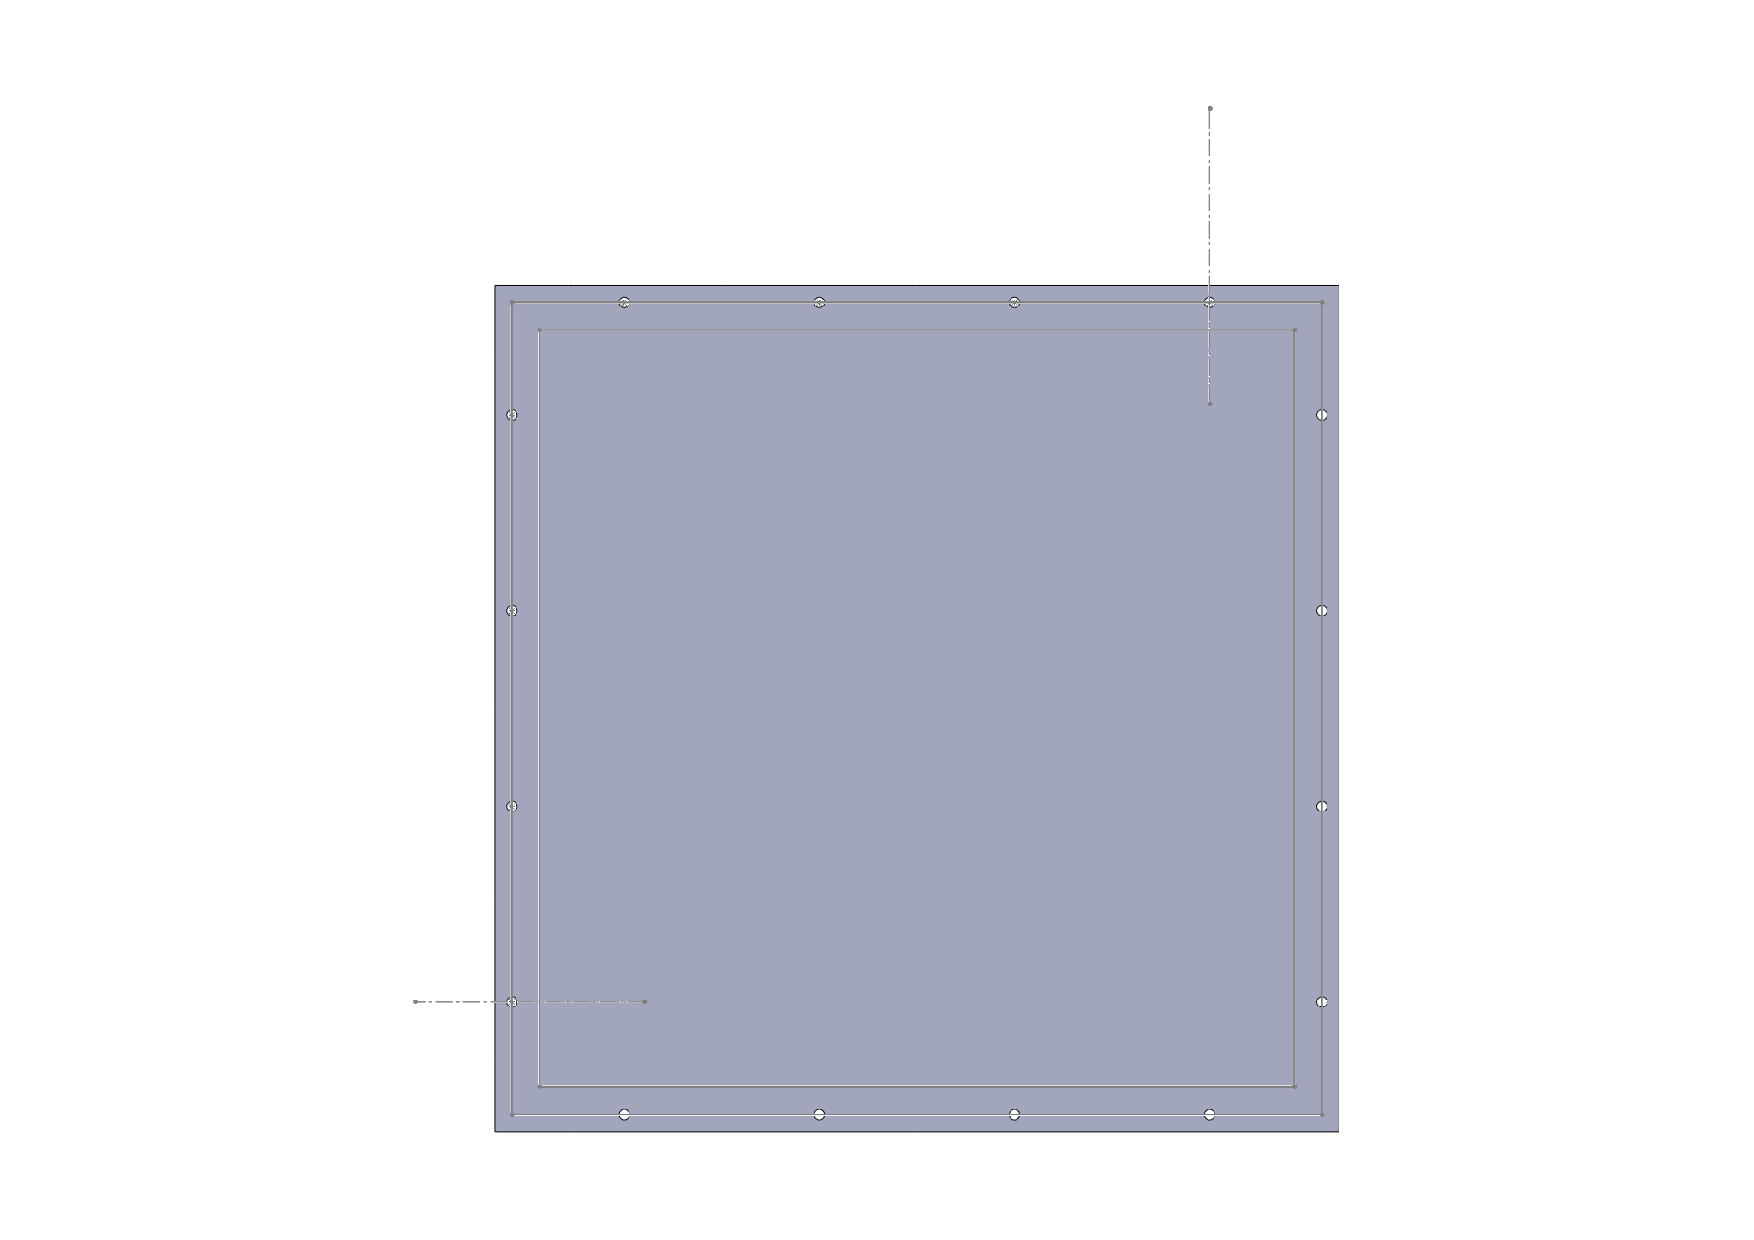
\includegraphics[width = \textwidth]{assets/Annexes/chablon trous.pdf}
\end{figure}
\includepdf[pages=2-,scale=0.9,pagecommand={}]{assets/Annexes/UVLS-Clears-TDS.pdf}

\newpage
\section[Chablon trous vitre]{Chablon trous fixation vitre}\label{chablon_trous_vitre}

\begin{figure}[H]
    \centering
    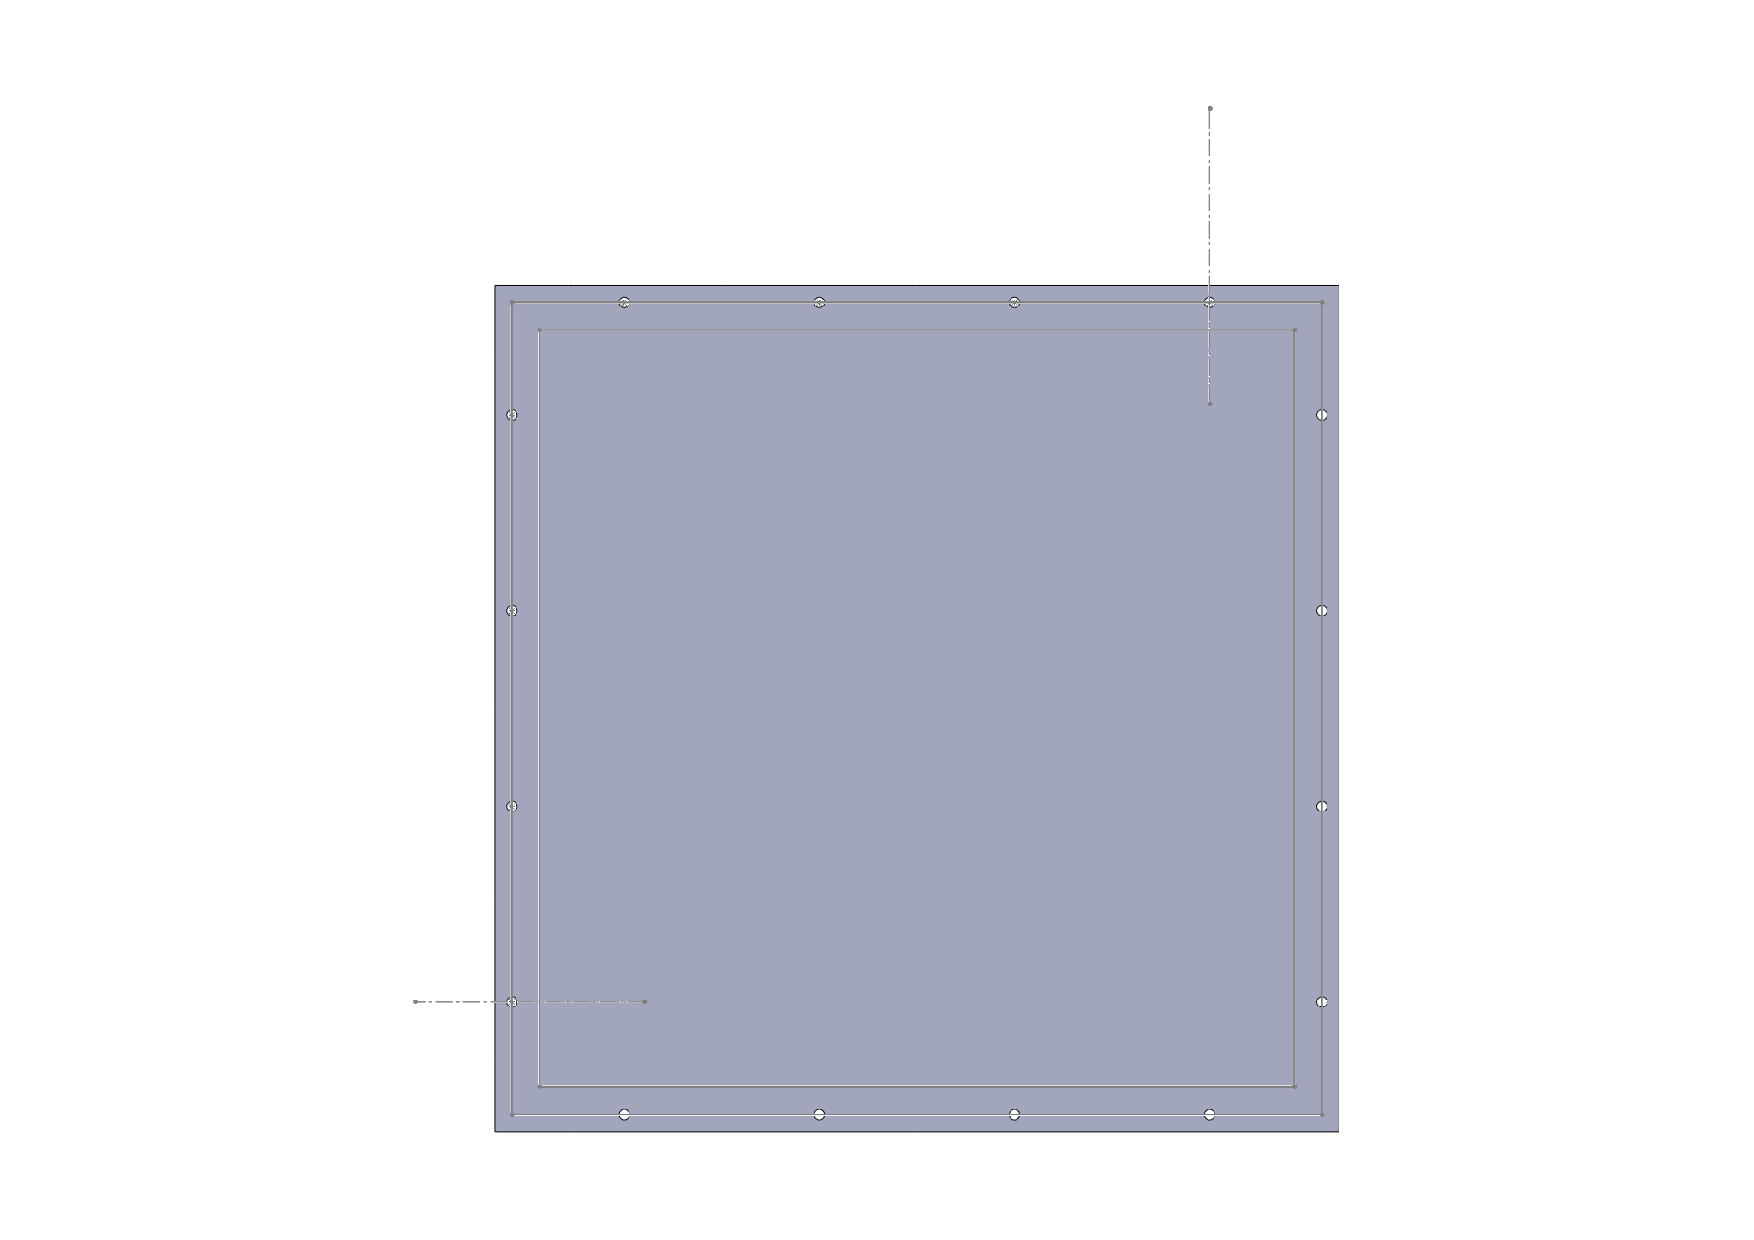
\includepdf[pages=-,scale=1,pagecommand={}]{assets/Annexes/chablon trous.pdf}
    %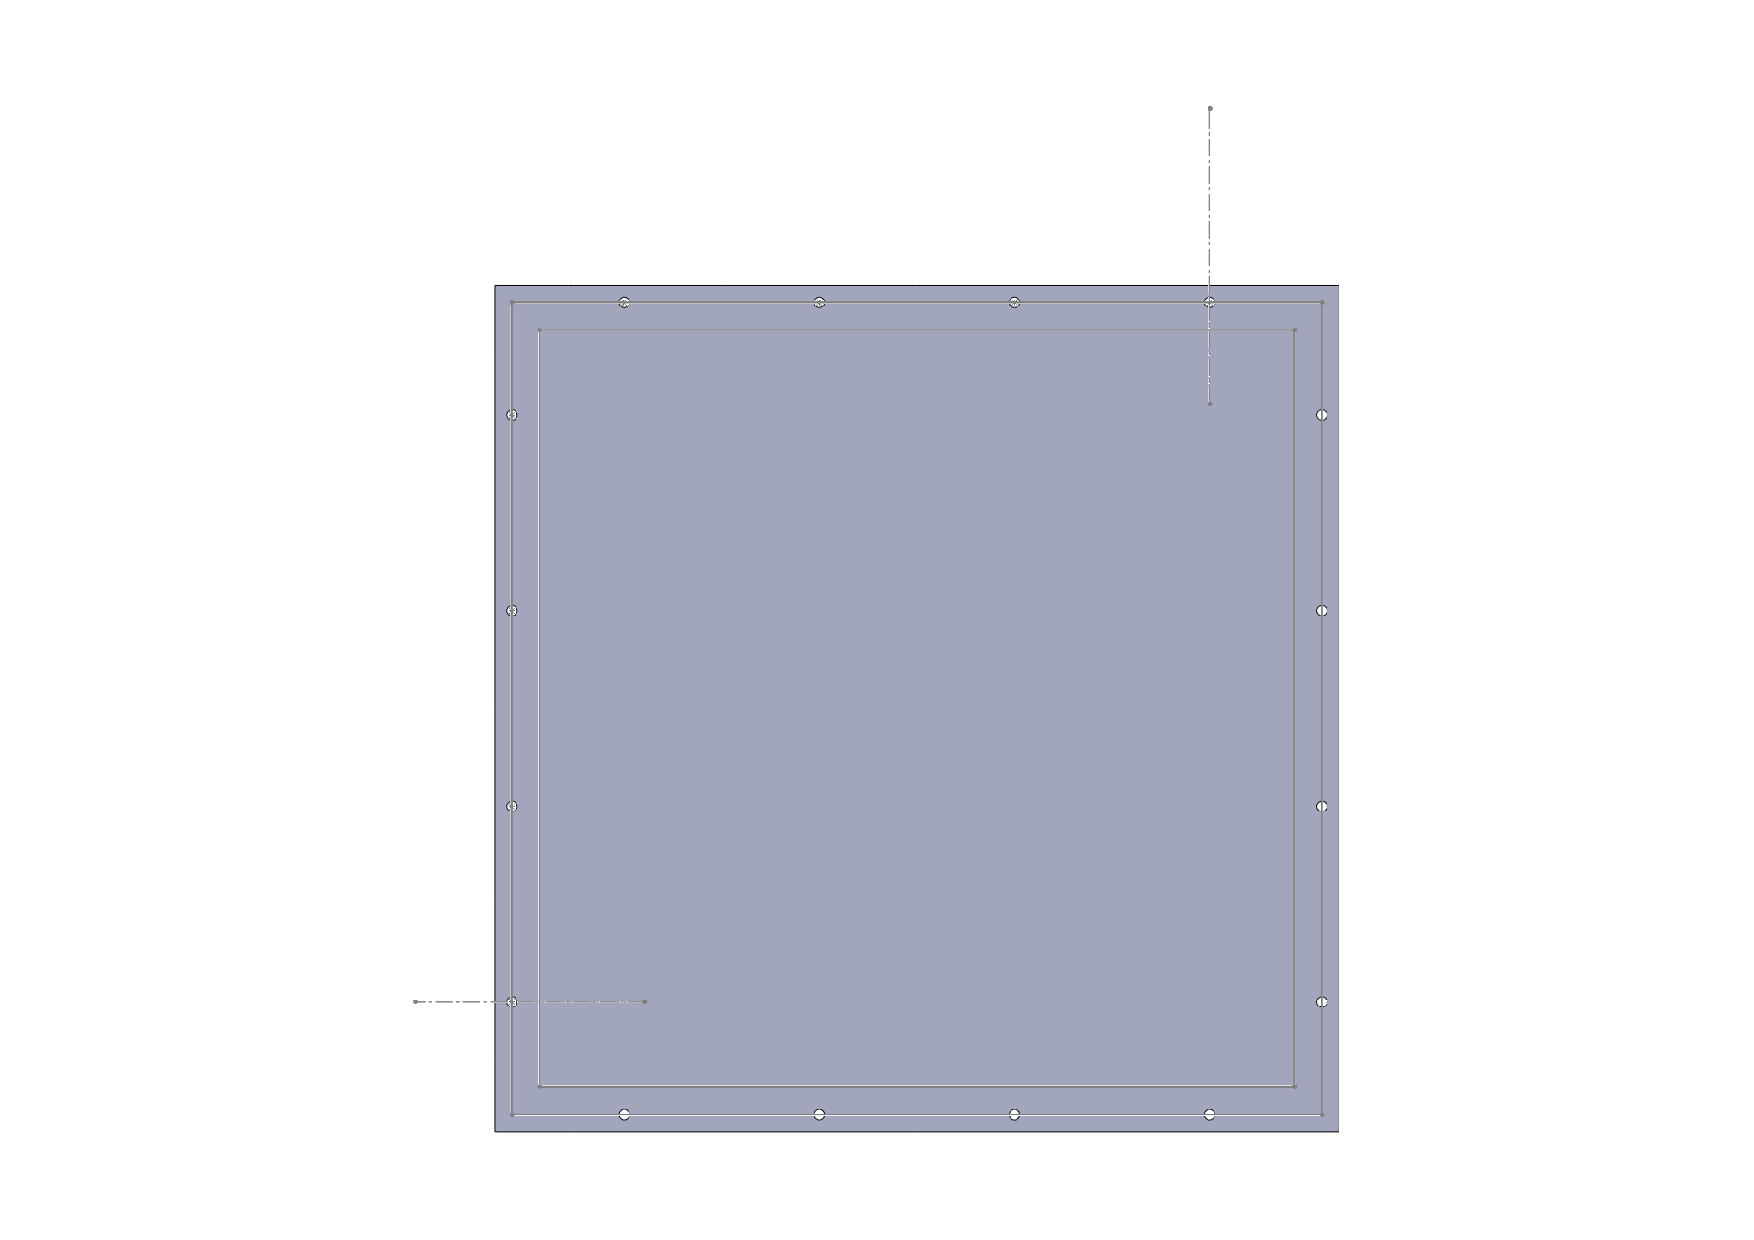
\includegraphics[width = \textwidth]{assets/Annexes/chablon trous.pdf}
\end{figure}
\footnotetext{Télécharger fichiers source \href{https://1drv.ms/f/s!Altwa7Vt0GlIjv5WyyjY6xfEgrsDBQ?e=dFzJzf}{ici}}

\newpage
\section[Code arduino mesure]{Code arduino mesure \href{https://1drv.ms/f/s!Altwa7Vt0GlIj4Bf6049yvu0P-8YLQ?e=v7KWOI}{télécharger}}\label{code:arduino_mesure}
\lstinputlisting[language=Arduino]{assets/code/Code_arduino_mesure.ino}
\footnotetext{Télécharger fichiers source \href{https://1drv.ms/f/s!Altwa7Vt0GlIj4Bf6049yvu0P-8YLQ?e=v7KWOI}{ici}}


\section[Diagramme électrique PCB mesure]{Diagramme électrique PCB mesure\href{https://1drv.ms/f/s!Altwa7Vt0GlIjv0bGlDjWqrtS53P8w?e=SVTypX}{Télécharger}}\label{PCB:mesure}
\begin{figure}[H]
    \centering
    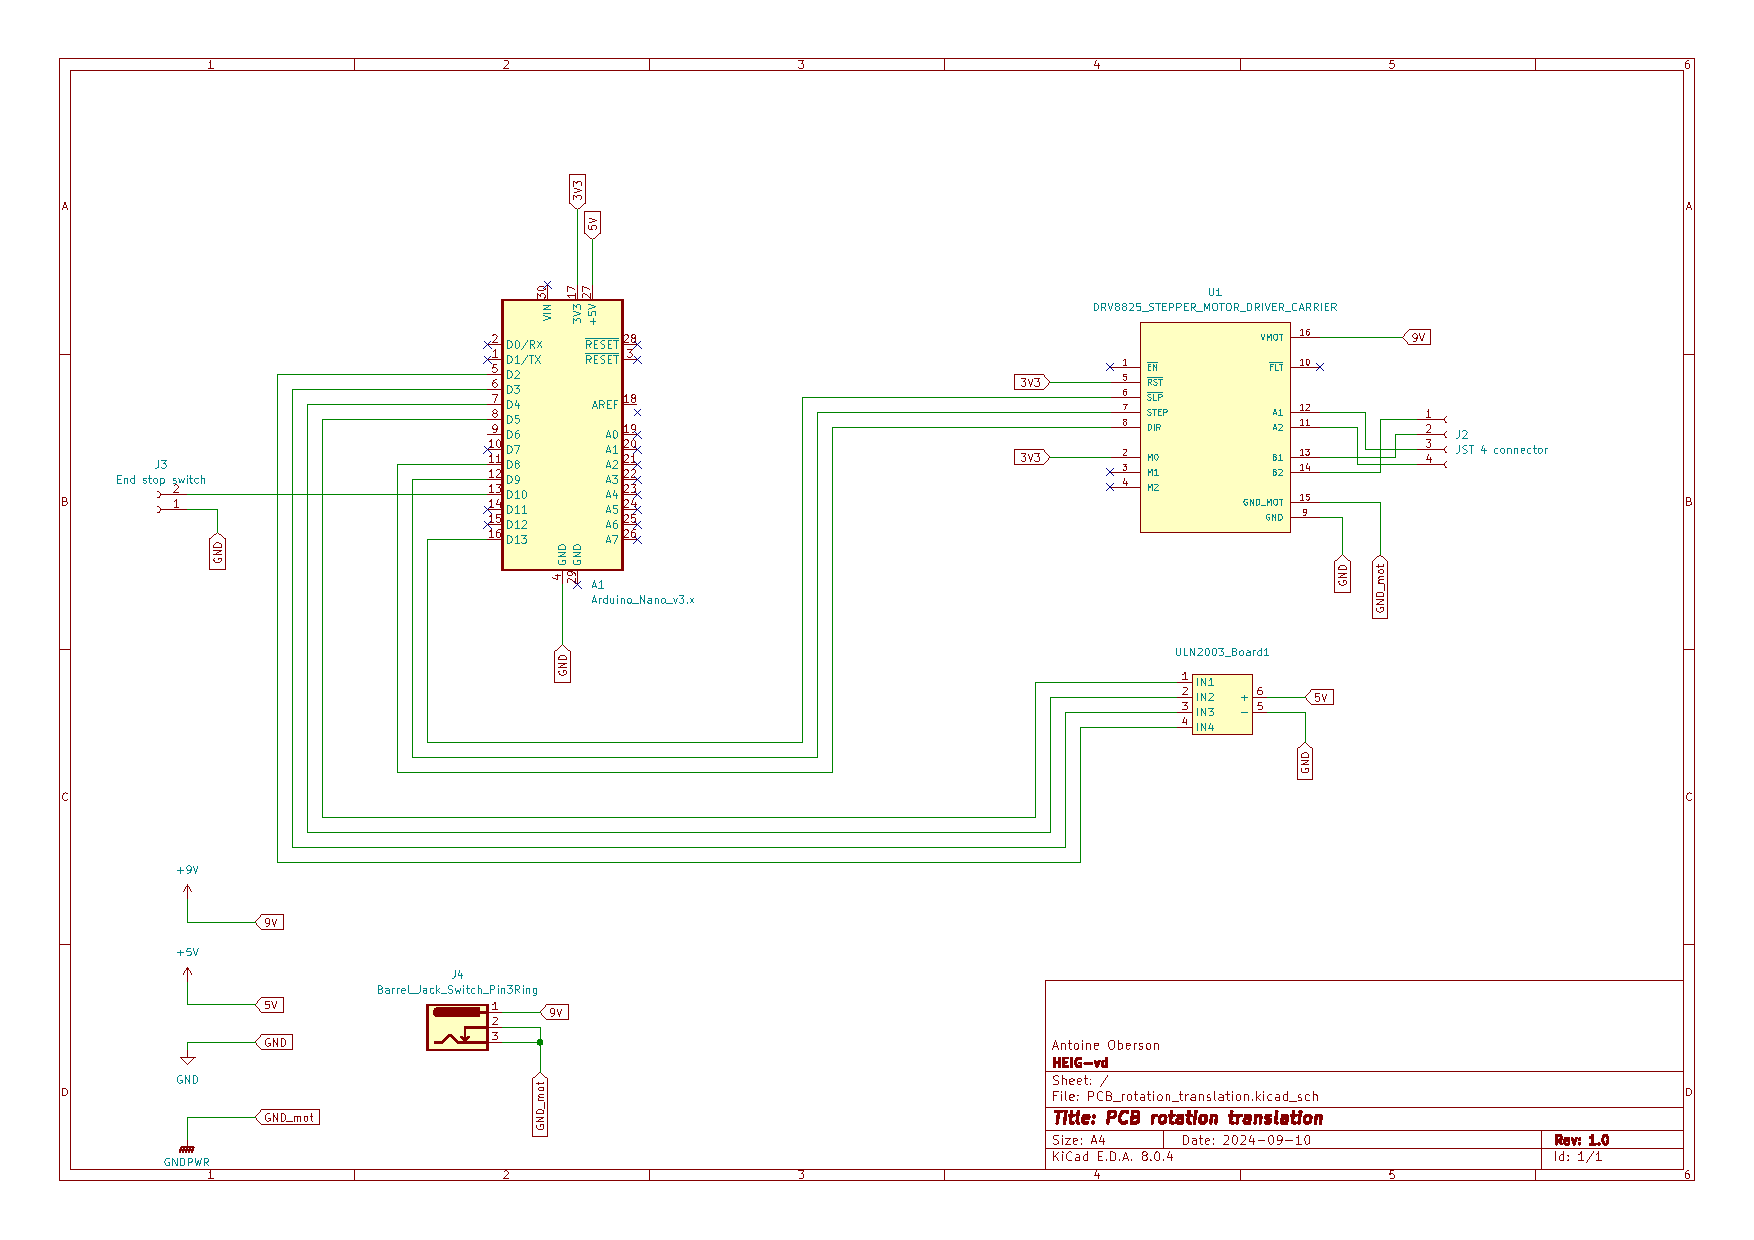
\includegraphics[angle = 90,height = 0.8\paperheight]{assets/Annexes/PCB_rotation_translation_diagramme_elec.pdf}
    %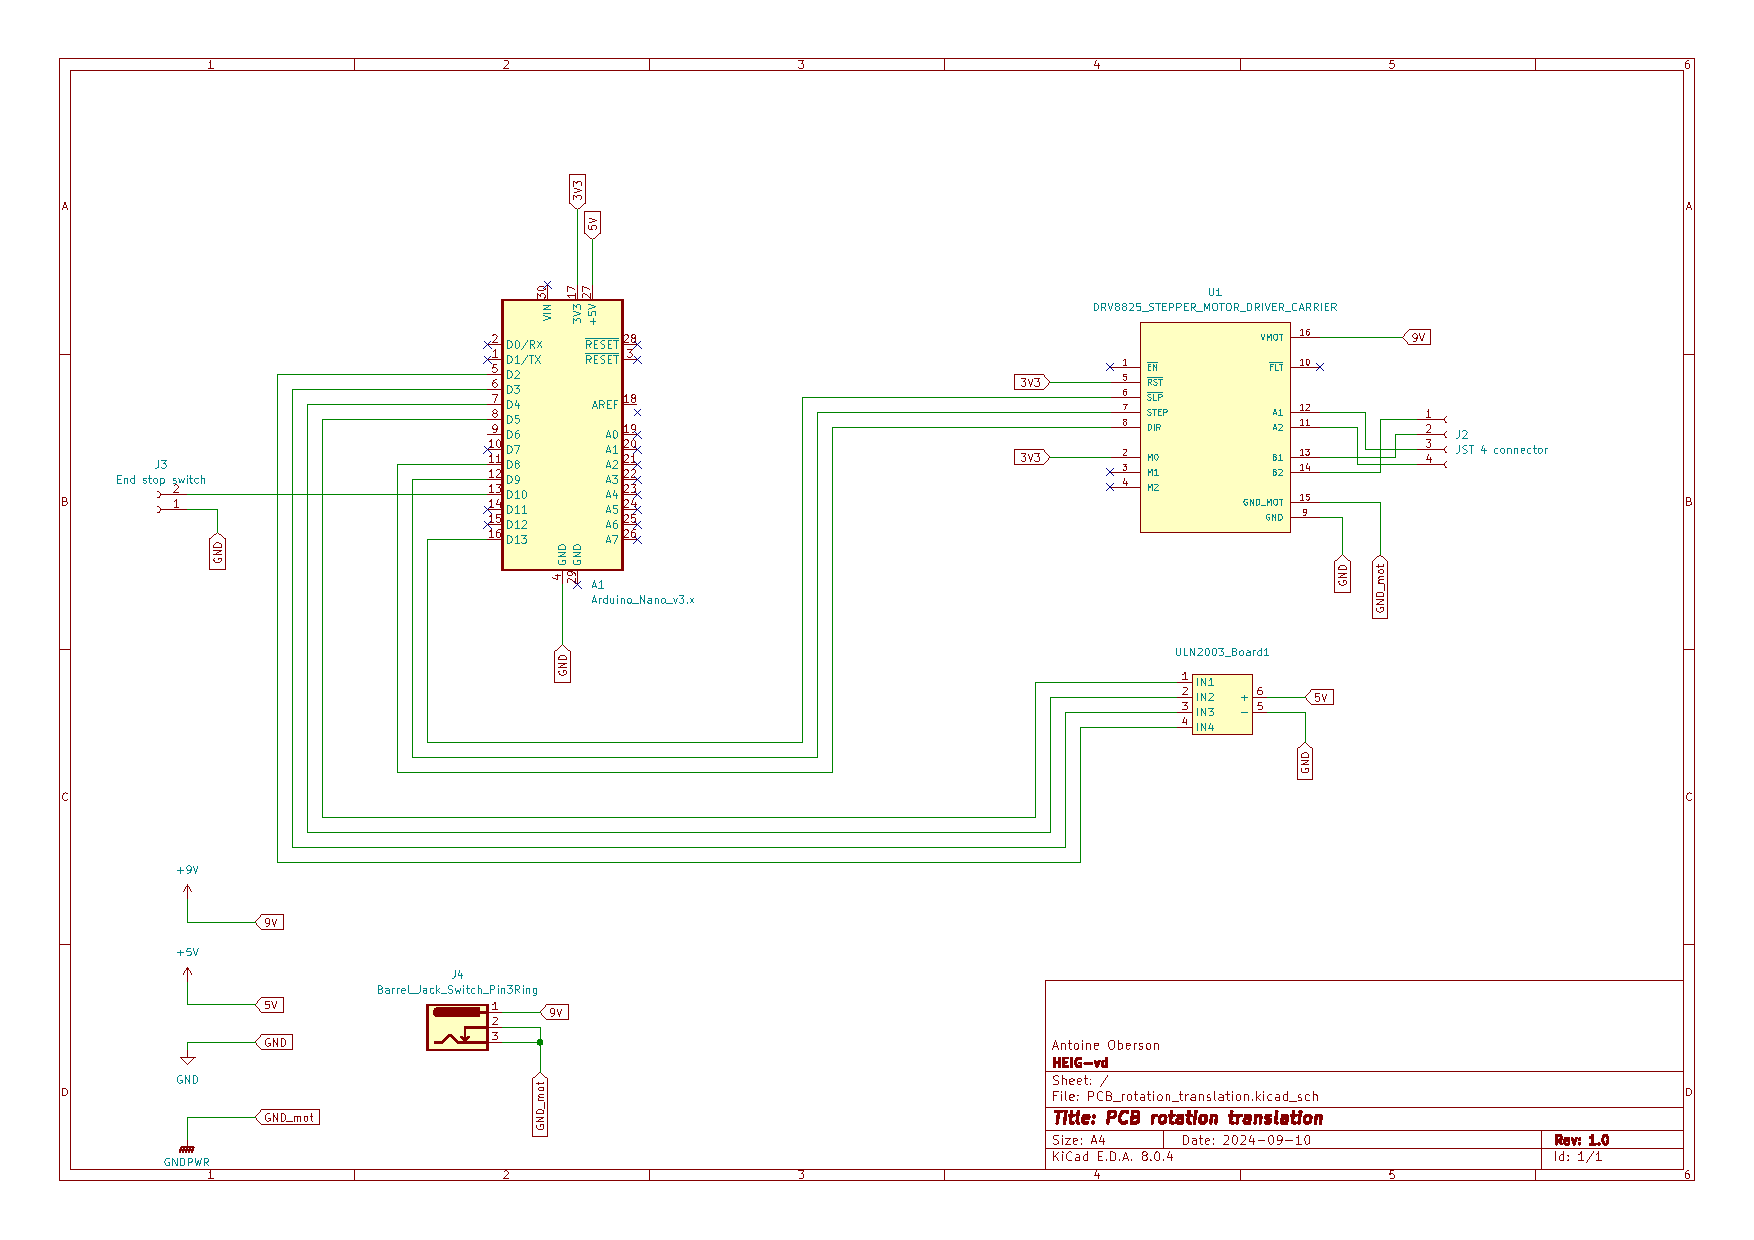
\includepdf[pages=-,scale=1,angle = 90,pagecommand={}]{assets/Annexes/PCB_rotation_translation_diagramme_elec.pdf}
    %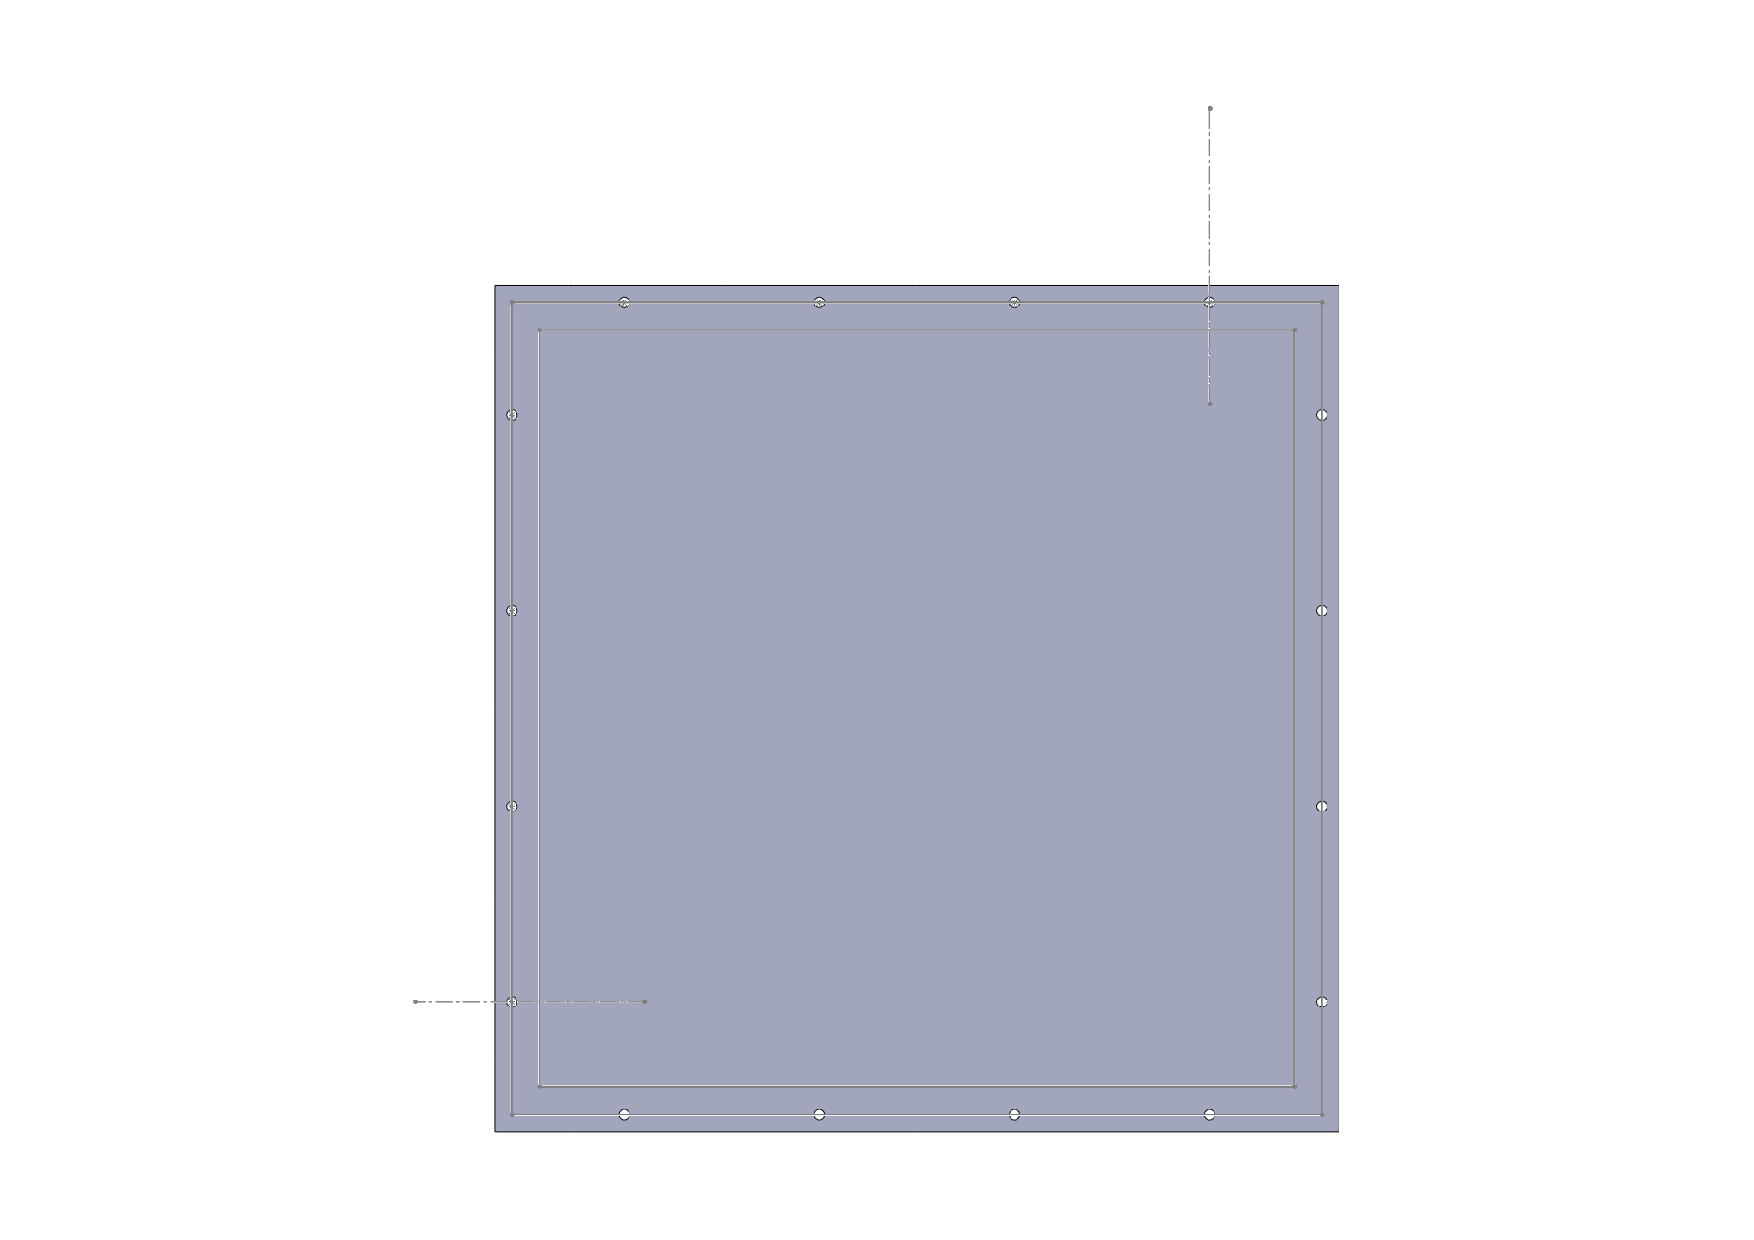
\includegraphics[width = \textwidth]{assets/Annexes/chablon trous.pdf}
\end{figure}

\section[Mise en plan Système de mesure]{Mise en plan Système de mesure}\label{mise_en_plan_systeme_mesure}

\begin{figure}[H]
    \centering
    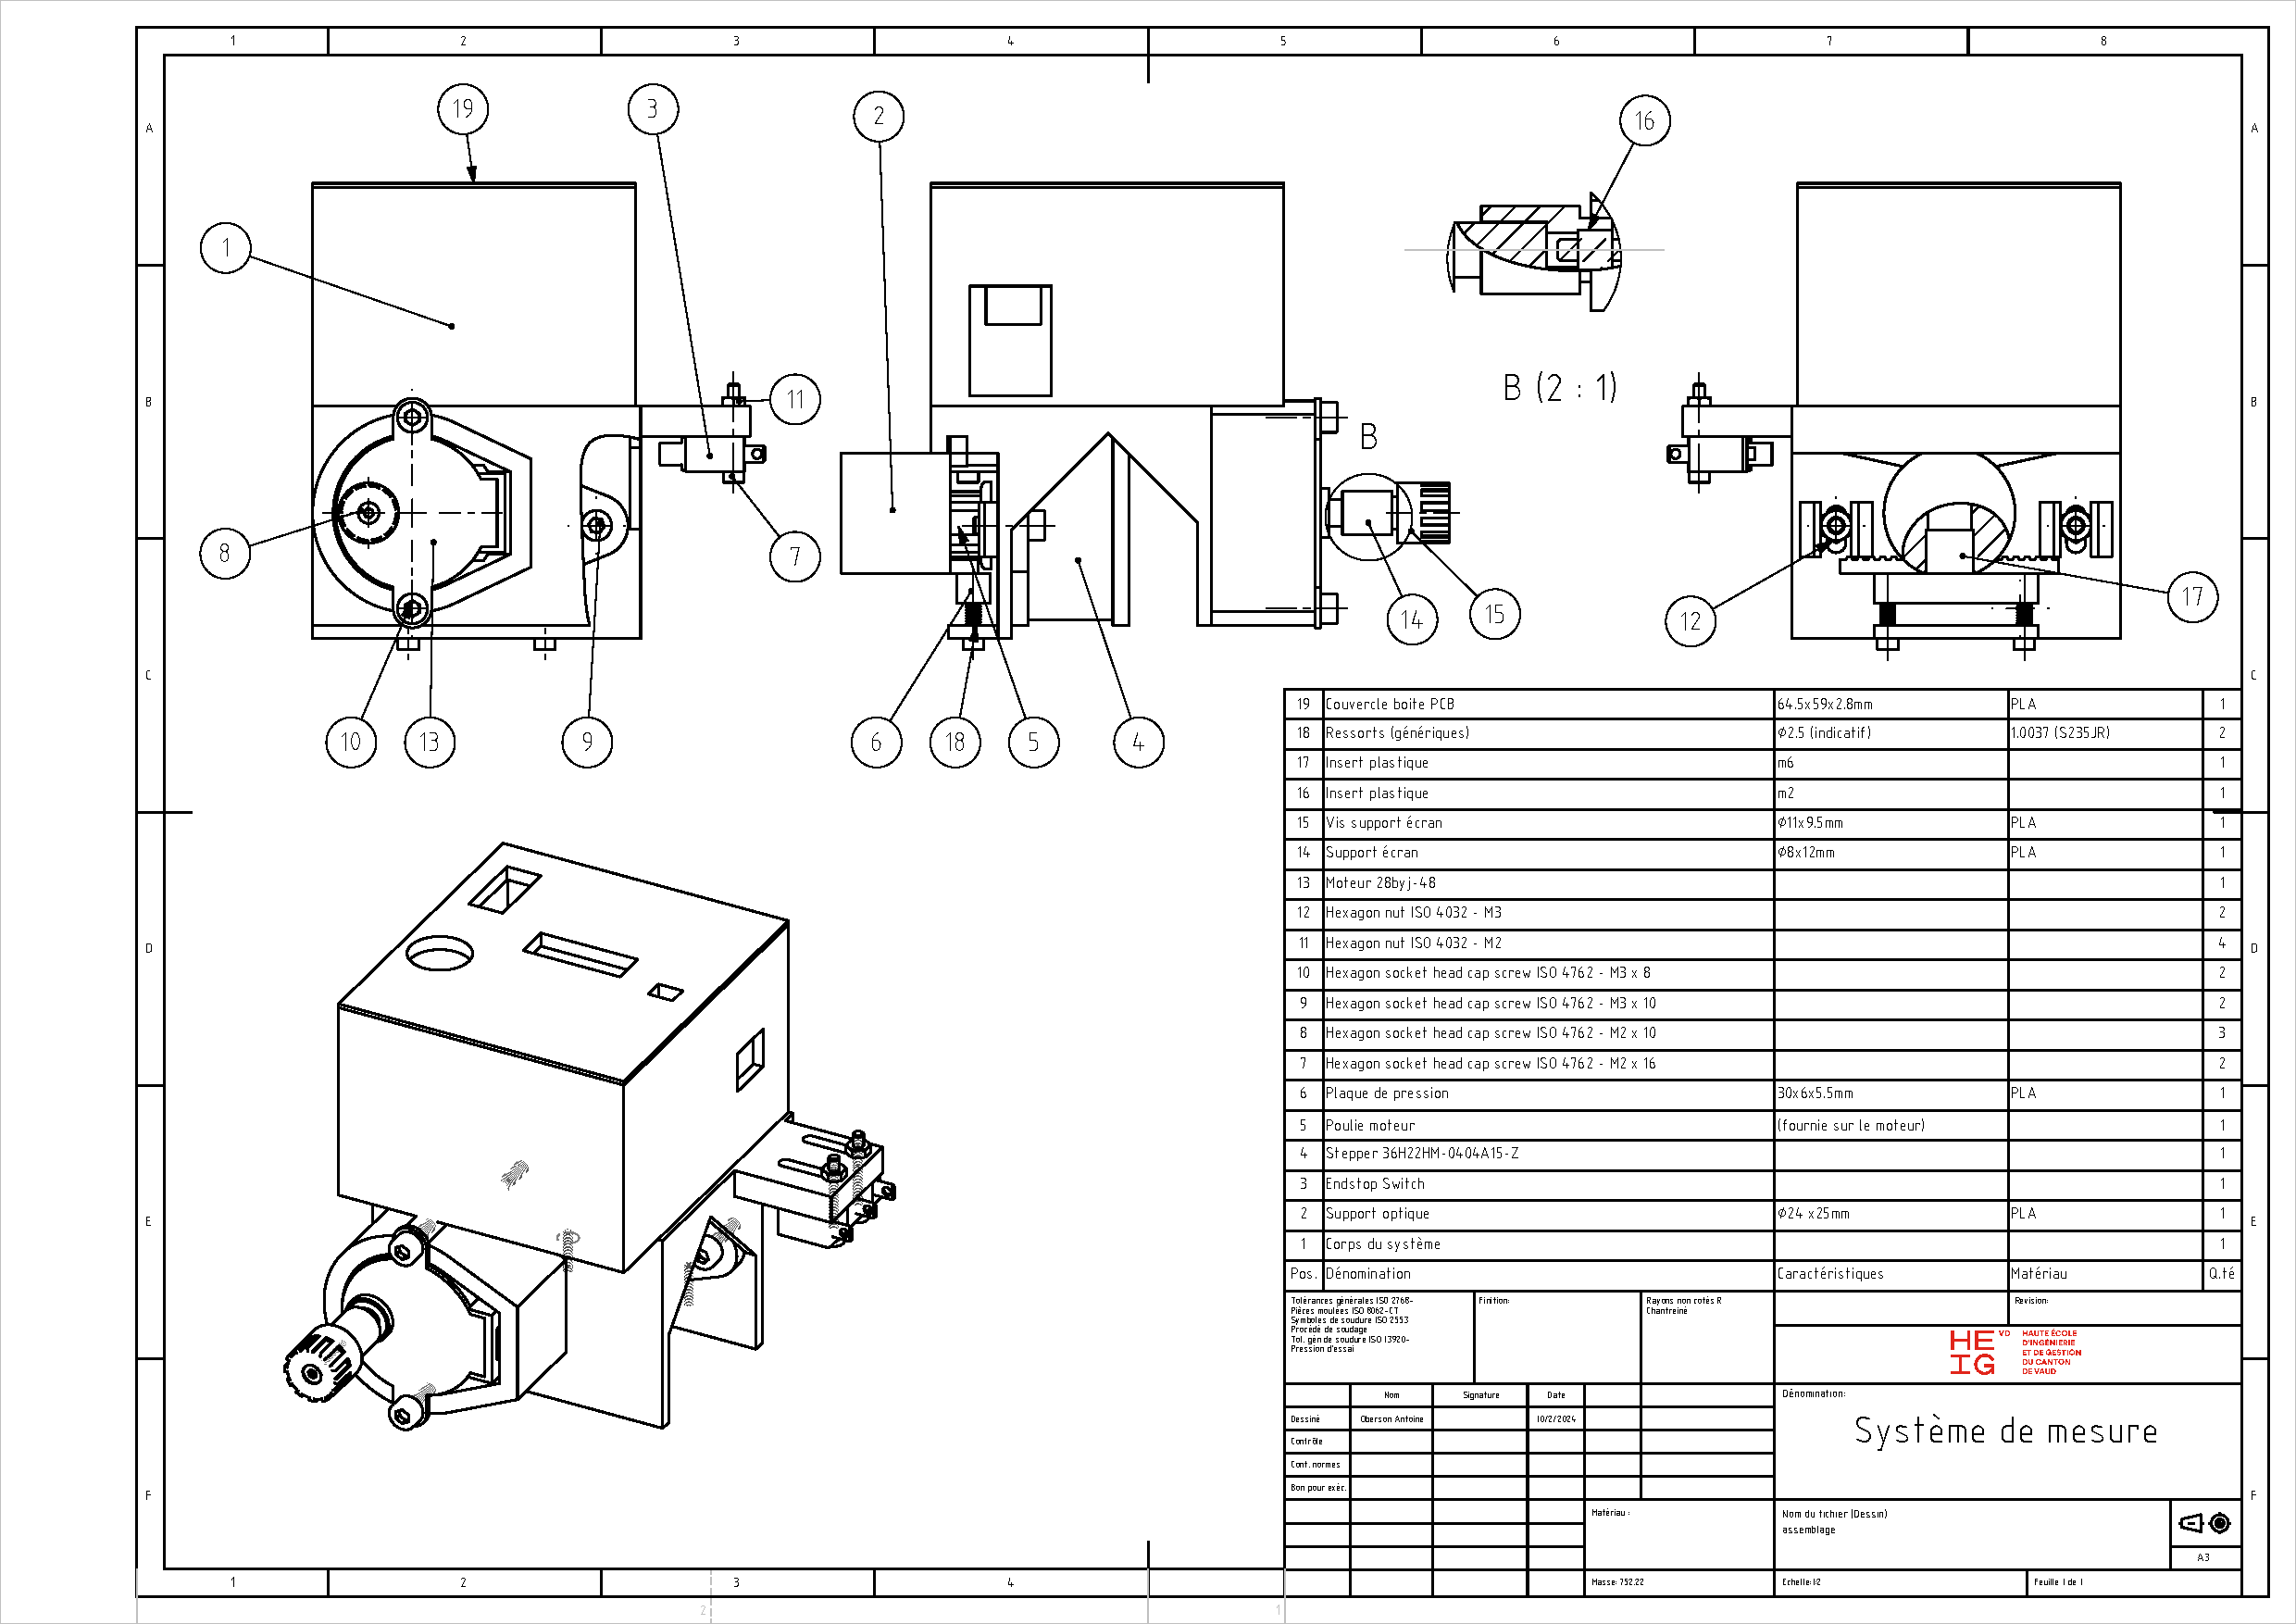
\includepdf[pages=-,scale=0.7,angle = 90,pagecommand={}]{assets/Annexes/assemblage_machine_mesure.pdf}
    %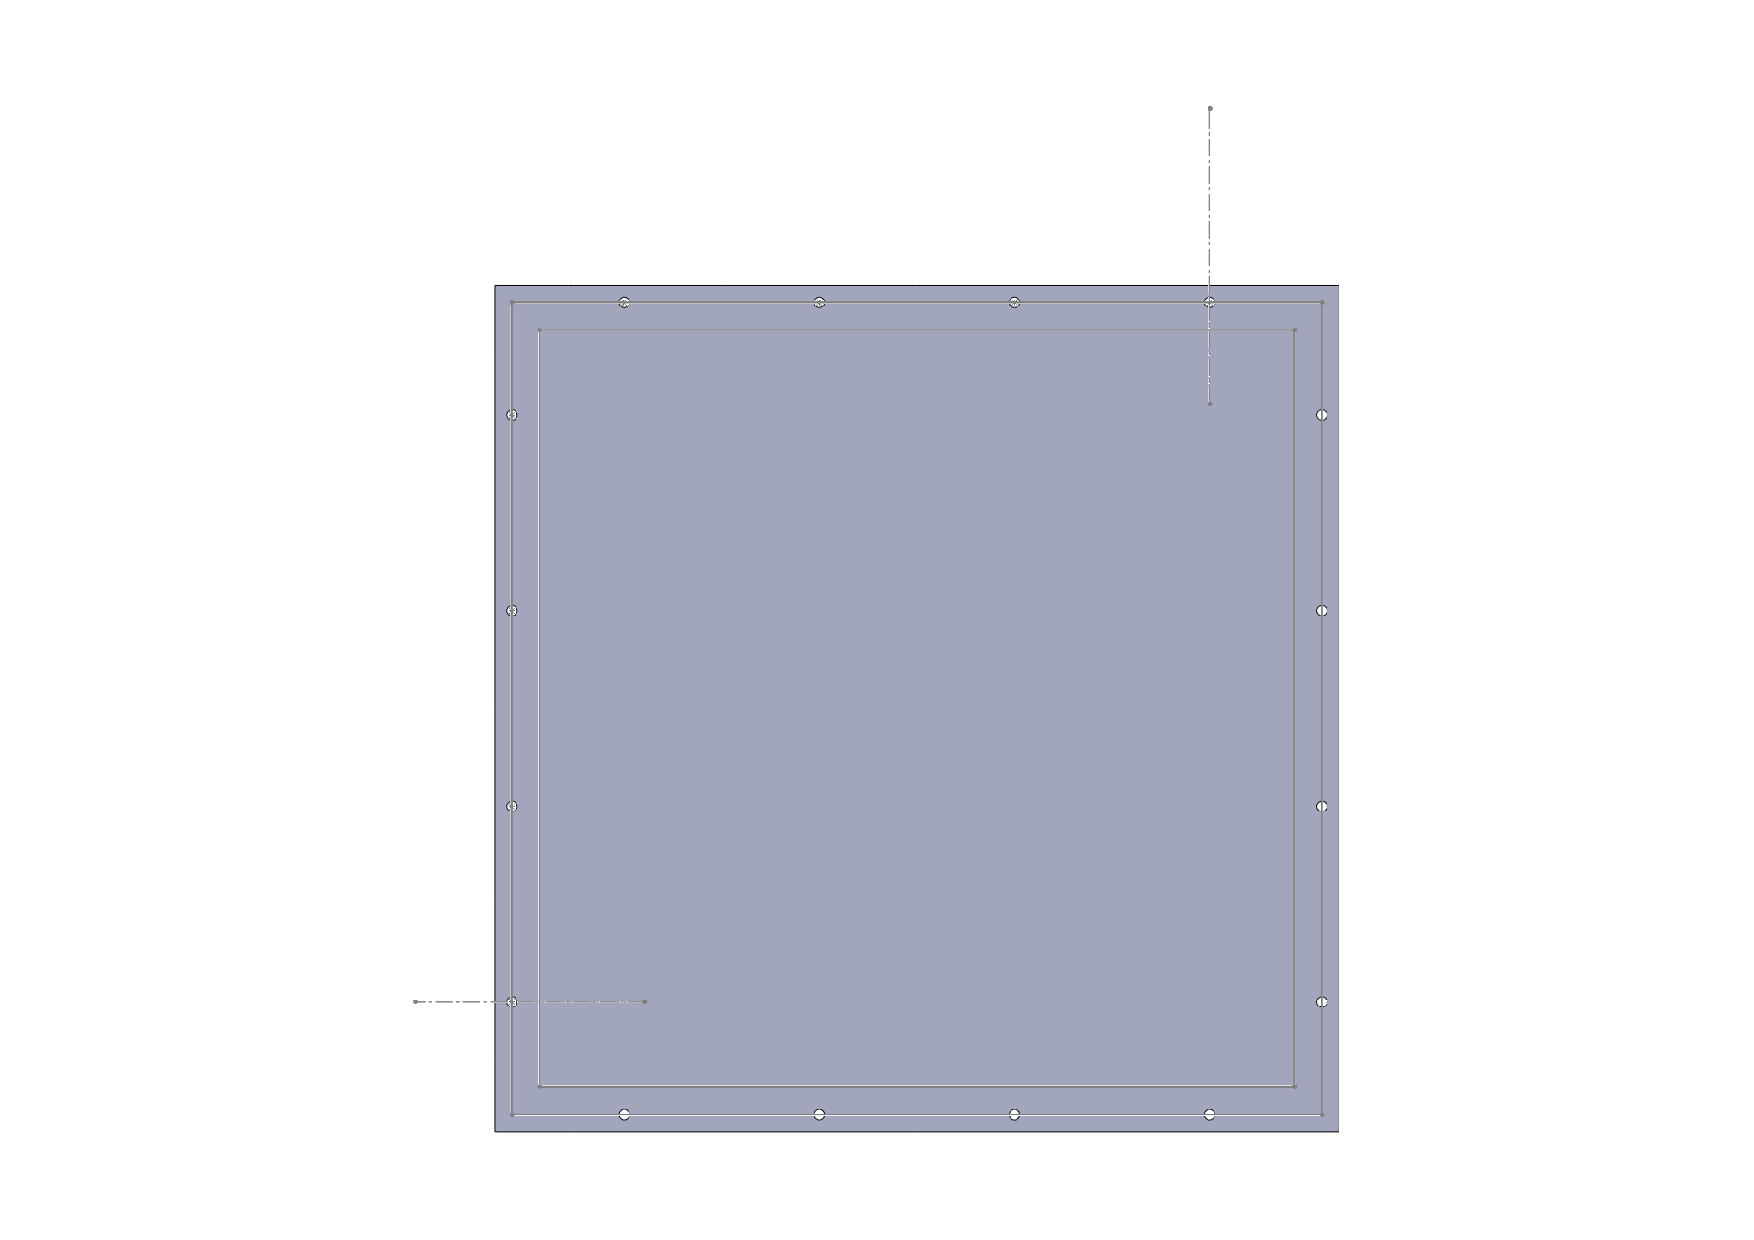
\includegraphics[width = \textwidth]{assets/Annexes/chablon trous.pdf}
\end{figure}